\newpage

\section{Simulation Analysis}
\label{sec:simulation}

\subsection{Operating Point Analysis - The given Circuit for $t<0$}

Table~\ref{tab:sim1} shows the simulated operating point results for the circuit under analysis, for $t<0$.

\begin{table}[htb!]
  \centering
  \begin{tabular}{|l|r|}
    \hline    
    {\bf Name} & {\bf Value [A or V]} \\ \hline
    @gb[i] & -2.48284e-04\\ \hline
@r1[i] & 2.369027e-04\\ \hline
@r2[i] & -2.48284e-04\\ \hline
@r3[i] & -1.13810e-05\\ \hline
@r4[i] & 1.210640e-03\\ \hline
@r5[i] & -2.48284e-04\\ \hline
@r6[i] & 9.737374e-04\\ \hline
@r7[i] & 9.737374e-04\\ \hline
v(1) & 5.185042e+00\\ \hline
v(2) & 4.941554e+00\\ \hline
v(3) & 4.425830e+00\\ \hline
v(5) & 4.977013e+00\\ \hline
v(6) & 5.729012e+00\\ \hline
v(7) & -1.97652e+00\\ \hline
v(8) & -2.95469e+00\\ \hline
v(9) & 0.000000e+00\\ \hline

  \end{tabular}
  \caption{Operating point results. A variable preceded by @ is of type {\em current}
    and expressed in Ampere; other variables are of type {\it voltage} and expressed in
    Volt.}
  \label{tab:sim1}
\end{table}

These results were produced using the \textit{Ngspice software}.

For this range of time, the circuit is time static, which means that the Capacitor C behaves as an open circuit. This is shown in Figure \ref{fig:sim1}.
As well as that modification, we also had to add a new Independent Voltage Source with a voltage of 0V whose current would be $I_d$, in order for \textit{Ngspice} to recognise the Current-Controlled Voltage Source, defined in Figure \ref{fig:sim1} as $H_d$. Bearing this in mind the Voltage Source was added between node 0 and a new node 9, with node 9 being placed between the GROUND and the first terminal of $R_6$.

\begin{figure}[h] \centering
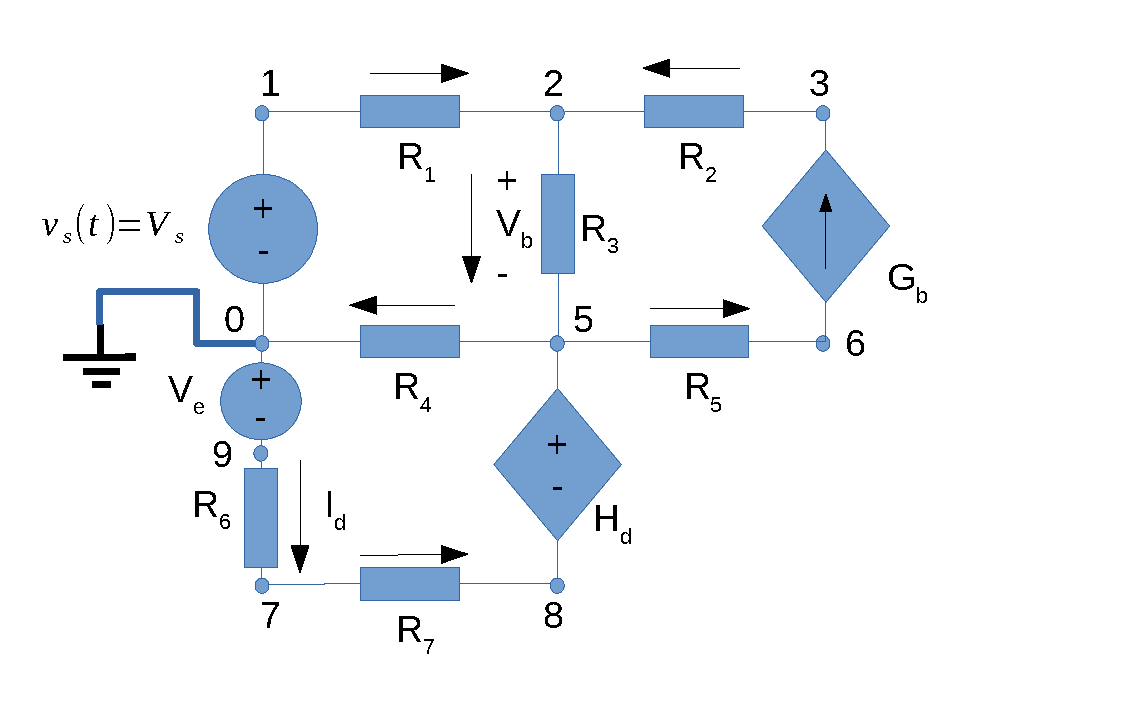
\includegraphics[width=0.4\linewidth]{t2-t-1-new-0V.pdf}
\caption{The original circuit with an added voltage source of value 0V.}
\label{fig:sim1}
\end{figure}

OP2

\begin{table}[htb!]
  \centering
  \begin{tabular}{|l|r|}
    \hline    
    {\bf Name} & {\bf Value [A or V]} \\ \hline
    @gb[i] & 3.571179e-18\\ \hline
@r1[i] & -3.40748e-18\\ \hline
@r2[i] & 3.571179e-18\\ \hline
@r3[i] & 1.636985e-19\\ \hline
@r4[i] & 7.278356e-19\\ \hline
@r5[i] & -2.86705e-03\\ \hline
@r6[i] & 5.854099e-19\\ \hline
@r7[i] & 5.854099e-19\\ \hline
v(2) & 3.502198e-15\\ \hline
v(3) & 1.092010e-14\\ \hline
v(5) & 2.992175e-15\\ \hline
v(6) & 8.683696e+00\\ \hline
v(7) & -1.18828e-15\\ \hline
v(8) & -1.77636e-15\\ \hline
v(9) & 0.000000e+00\\ \hline

  \end{tabular}
  \caption{Operating point results. A variable preceded by @ is of type {\em current}
    and expressed in Ampere; other variables are of type {\it voltage} and expressed in
    Volt.}
  \label{tab:op2}
\end{table}

\begin{figure}[h] \centering
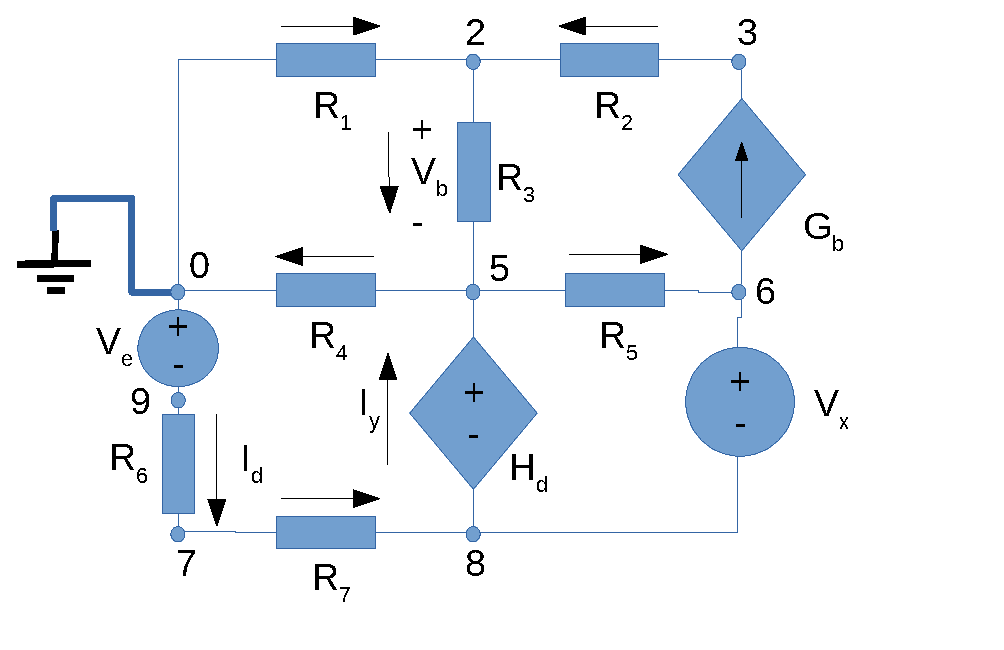
\includegraphics[width=0.4\linewidth]{t2-t-2-new-0V.pdf}
\caption{The original circuit with an added voltage source of value 0V.}
\label{fig3}
\end{figure}


To compare the results between the theoretical calculations and the simulation, it's important to keep in mind that the current values and directions represented in \ref{fig2} by round arrows: $I_1$, $I_2$, $I_3$ and $I_4$ correspond, respectively, to the following values in the simulation data table (\ref{tab:op}): @r1[i], -@r2[i], -@id[current], -@r6[i] (or @r7[i], they're equivalent).


On a general basis, the values obtained by the simulation greatly resemble the ones obtained using the theoretical models and the application \textit{GNUOctave} to compute them.

In fact, by inspection it's possible to conclude that pratically all the values fit in the same magnitude as its correspondent. 

As it's possible to check in the following table, the relative uncertainties ($|theoretical - simulated|/|theoretical|$) are considerably slim.
Although we have a rather significant uncertainty for the value of V7 (theoretical value: -9.7816698e-01 V , simulated value: 8.139731e+00 V, uncertainty: 2.0000000e+00); the smallest uncertainty, which null, reports to the value of $I_1$ (theoretical value: 2.3690260e-04 A , simulated value: 2.369026e-04 A). It's relevant to note that this number isn't actually zero, but instead, the program doesn't have enough precison to compute a detectable error. 

